\documentclass{beamer}
\usepackage{fontawesome}
\usepackage{hyperref}
\usetheme{Madrid}
\usecolortheme{sidebartab}
\usefonttheme{professionalfonts}
\urlstyle{same}

\title{Ansible for NetworkAutomation}
\date{2019-09}

\begin{document}

\frame{\titlepage}

\begin{frame}
    \frametitle{Session Overview}
    \tableofcontents
\end{frame}

\begin{frame}
\frametitle{Session Overview}
At the end of this session you will be able to:
\begin{itemize}
    
  \item <2-> Review the playbook management keys and values
  \begin{itemize}
    \item <3-> vars:
    \item <4-> connection:
    \item <5-> hosts:
  \end{itemize}
  \item <6-> Update an Ansible config file to manipulate playbook wide settings
  \item <7-> Gather data from various devices
    \begin{itemize}
        \item IOS
        \item NXOS
        \item Juniper
        \item Other network devices
    \end{itemize}
  \item <8-> Use regex to parse data from a command with data gathered
\end{itemize}
\end{frame}

\begin{frame}
\frametitle{Network Diagram}
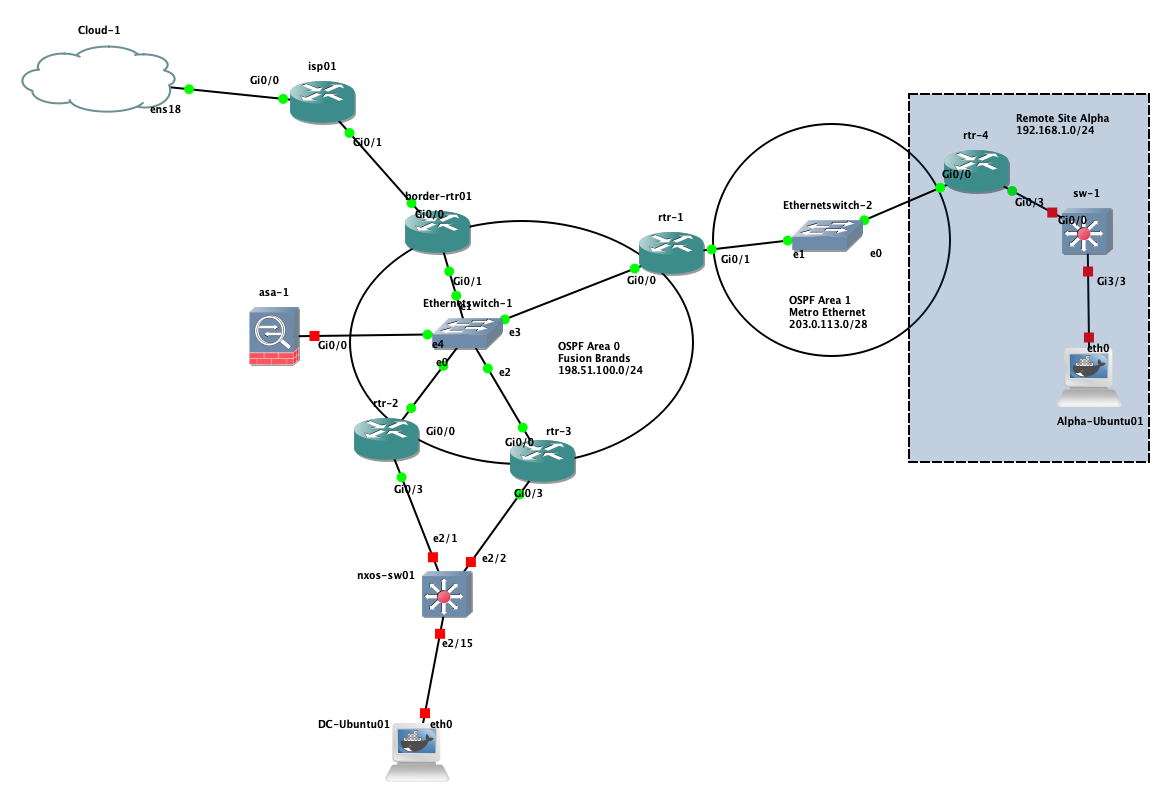
\includegraphics[width=\textwidth]{assets/base_setup.png}
\end{frame}

\begin{frame}[fragile]
    \frametitle{Playbook Management Key Values}
    All Ansible playbooks are defined within YAML format, which leverages key/value
    pair assignments. We will take a look at some common keys used, and what their
    corresponding value looks like.
\begin{verbatim}
- name: "PLAY 1: Gather data from router"
  connection: network_cli
  hosts: r1
  become: true
  become_method: enable
\end{verbatim}
\end{frame}

\begin{frame}
  \frametitle{Quick Note on Ansible Modules}
  \begin{block}{Ansible Network Modules}
    The whole list of Network modules and their corresponding requirements
    can be found with your favorite search engine on term of "Ansible Network Modules" 
    - which will take you to this link: \url{https://docs.ansible.com/ansible/latest/modules/list_of_network_modules.html}
    This will be included on the notes for this.
    \end{block}
\end{frame}

\begin{frame}
    \frametitle{Gathering Data from Cisco IOS Devices}
    There are two primary methods to gather data from IOS devices, using:
    \begin{itemize}
        \item<2-> \textbf{cli\_command}
        \item<3-> \textbf{ios\_command}
        \item<4-> More modules for interacting with IOS devices can be found on the Ansible Network Modules Page
    \end{itemize}
\end{frame}

\begin{frame}
    \frametitle{ios\_command}
    This is used when working with Cisco IOS devices connecting with SSH.
    
\end{frame}


\end{document}